% !TEX root = ../../../main.tex
% 来源：中学数学实验教材·第二册（几何）
% 章节：直线形 / 相似形
% 原始文件：3.tex，行 5642-5649
% 类型：tikz
% ---
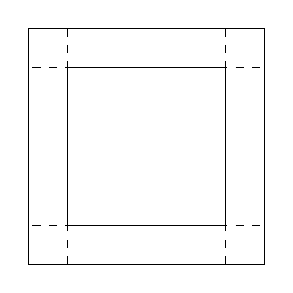
\begin{tikzpicture}
\draw(0,0) rectangle (3,3);
\draw(.5,.5) rectangle (3-.5,3-.5);
\draw[dashed](.5,0)--(.5,.5)--(0,.5);
\draw[dashed](3-.5,0)--(3-.5,.5)--(3,.5);
\draw[dashed](.5,3)--(.5,3-.5)--(0,3-.5);
\draw[dashed](3-.5,3)--(3-.5,3-.5)--(3,3-.5);
\end{tikzpicture}
